% !TEX root = main.tex

\begin{quote}
    \em
    \vphantom{}\marginnote{%
        \textbf{หมายเหตุ}\; โจทย์บางข้อที่ปรากฏอาจมีลักษณะเป็นคำถามปรนัย (มีตัวเลือก)
        เนื่องจากเป็นข้อจำกัดของระบบในการแข่งขันระดับ Audition
    }%
    \llap{\adfdownleafleft\;}โจทย์ Quickfire เป็นโจทย์ประเภทถามเร็ว-ตอบเร็ว
    ผู้เข้าแข่งขันมีเวลา 10{\hrsp--\hrsp}60 วินาที ที่จะตอบคำถามให้ถูกต้อง
    โดยไม่สามารถใช้คอมพิวเตอร์เพื่อช่วยหาคำตอบได้
\end{quote}

\question{\label{q:quickfire-central-audition-linearswap}}

จงพิจารณาโปรแกรมดังต่อไปนี้
\begin{lstlisting}
function mystery_<%\ref*{q:quickfire-central-audition-linearswap}%>(A[0...n-1]):
    # A <%\codecmt คือ%> 0-indexed array <%\codecmt ของจำนวนเต็ม%>
    n := A.length()
    for i := 0 to n-2 do:
        if A[i] > A[i+1] then:
            swap A[i] with A[i+1]
        end
    end
    return A
end
\end{lstlisting}

\medskip\noindent
จากโปรแกรมข้างต้นนี้ ประพจน์ใดกล่าวถูกต้อง\uline{บ้าง}?

\begin{enumerate}[label={$\square$}]
    \item \textbf{ประพจน์ P:} มีค่าค่าหนึ่งใน output array ซึ่งเมื่อลบออกจาก array ดังกล่าว จะทำให้ array ผลลัพธ์เป็น array ที่เรียงลำดับ
    \item \textbf{ประพจน์ Q:} สำหรับ input array A ใด ๆ ที่มีขนาด N จะได้ว่า \lstinline{f(A)[N-1] = max(A)}
    \item \textbf{ประพจน์ R:} สำหรับ input array A ใด ๆ ที่มีขนาด N จะได้ว่า \lstinline{f(A)[0] = min(A)}
\end{enumerate}

\question{}

ให้พิจารณาลำดับจำนวน Fibonacci ที่มีความยาวเป็นอนันต์\;
จงหาอัตราส่วนของ\uline{จำนวนเลขคู่}ต่อ\uline{จำนวนเลขคี่}ในลำดับจำนวนนี้

\question{}

ธนาคารกสิกรจัดประเพณีวิ่งควายที่จังหวัดชลบุรี มีควายร่วมเข้าแข่งขันวิ่งจำนวน 66 ตัว 
แต่ภายในงานมีลู่ให้ควายวิ่งได้แค่รอบละ 6 ตัวเท่านั้น

หากธนาคารต้องการหาควายที่วิ่ง\uline{เร็วที่สุด} 1 ตัว 
เราจะต้องนำควายมาจัดวิ่งแข่งกันทั้งหมดอย่างน้อยกี่รอบ?\hrsp%
\sidenote{%
    \textbf{เงื่อนไข}\; สมมติว่าควายวิ่งด้วยอัตราเร็วเท่าเดิมตลอดทุกรอบ 
    และเราไม่สามารถใช้นาฬิกาจับเวลาได้ แต่สามารถเปรียบเทียบได้ว่าในการแข่งขันรอบหนึ่ง ควายตัวใดเข้าเส้นชัยก่อนหรือหลังได้
}


\newpage
\question{}

ธนาคารกสิกรจัดประเพณีวิ่งควายที่จังหวัดชลบุรี มีควายร่วมเข้าแข่งขันวิ่งจำนวน 45 ตัว 
แต่ภายในงานมีลู่ให้ควายวิ่งได้แค่รอบละ 5 ตัวเท่านั้น

หากธนาคารต้องการหาควายที่วิ่ง\uline{เร็วที่สุด}และ\uline{ช้าที่สุด} อย่างละ 1 ตัว เราจะต้องนำควายมาจัดวิ่งแข่งกันทั้งหมดอย่างน้อยกี่รอบ?

\question{}

กำหนดให้มีต้นไม้ค้นหาแบบทวิภาค (Binary search tree) ที่\uline{ว่างเปล่า}อยู่ต้นหนึ่ง\;
จากนั้นเรา insert ข้อมูลจำนวนเต็ม 9, 2, 3, 4, 18, 11, 20 เข้าไปในต้นไม้นี้ตามลำดับ 
โดยที่\uline{ไม่เกิด}กระบวนการ tree rebalancing ขึ้น

จงหาความสูง (height) ของต้นไม้ผลลัพธ์\;
(\textbf{หมายเหตุ:} กำหนดให้ Binary search tree ที่มี node เดียวมีความสูงเท่ากับ 0)

\question{}

สมมติว่ามี array ของจำนวนเต็มที่\uline{เรียงลำดับแล้ว} ขั้นตอนวิธีใดต่อไปนี้กระทำได้เร็วที่สุด?

\begin{enumerate}[label={$\Circle$}]
\item ค้นหาตัวเลข 42 ว่าอยู่ใน array หรือไม่
\item นับว่ามีจำนวนตัวเลขที่แตกต่างกันภายใน array ทั้งหมดกี่ตัว
\item หาค่าเฉลี่ยเลขคณิต (Arithmetic mean) ของตัวเลขทั้งหมดใน array
\item นับว่ามีเลขคู่ทั้งหมดกี่ตัวใน array
\item ทุกคำตอบข้างต้นใช้เวลาเป็น linear เท่ากันหมด ดังนั้นจึงใช้เวลาพอ ๆ กัน
\end{enumerate}

\question{}

จงพิจารณาโปรแกรมดังต่อไปนี้ที่เขียนขึ้นเพื่อนับว่า 
มีจำนวนคู่กี่จำนวนในบรรดาจำนวนตั้งแต่จำนวนเต็ม \lstinline{m} จนถึงจำนวนเต็ม \lstinline{n} (สมมติว่า \verb|m ≤ n|)\;
โปรแกรมนี้จะให้ผลลัพธ์ที่\uline{ถูกต้อง}ภายใต้เงื่อนไขใดของ input \uline{บ้าง}?
\begin{lstlisting}
function count_even(m, n):
    # m, n <%\codecmt คือจำนวนเต็มซึ่ง%> m <= n
    count := 0
    i := m
    while i <= n do:
        count := count + 1
        i := i + 2
    end
    return count
end
\end{lstlisting}

\begin{multicols}{2}
\begin{itemize}[label={$\square$}]
    \item กรณีที่ \verb|m| และ \verb|n| เป็นจำนวนคู่
    \item กรณีที่ \verb|m| เป็นจำนวนคี่ \verb|n| เป็นจำนวนคู่
    \item กรณีที่ \verb|m| เป็นจำนวนคู่ \verb|n| เป็นจำนวนคี่
    \item กรณีที่ \verb|m| และ \verb|n| เป็นจำนวนคี่
\end{itemize}
\end{multicols}
\question{}

ธนาคารกสิกรไทยสาขาหนึ่งเปิดให้บริการตั้งแต่เวลา 8:30 จนถึง 15:30 ของวันเดียวกัน\;
อยากทราบว่าในช่วงเวลาดังกล่าวจะมีเหตุการณ์ที่เข็มสั้นและเข็มยาวของนาฬิกาทำมุม%
\uline{ตั้งฉากกันพอดี}ทั้งหมดกี่ครั้ง?\hrsp%
\sidenote{%
    \textbf{เงื่อนไข}\; กำหนดให้เข็มสั้นและเข็มยาวขยับอย่างต่อเนื่องตลอดเวลา
}

\newpage
\question{\label{q:quickfire-northeast-audition-ec868bd3}}

จงพิจารณาโปรแกรมดังต่อไปนี้
\begin{lstlisting}
function mystery_<%\ref*{q:quickfire-northeast-audition-ec868bd3}%>(I):
   # I <%\codecmt คือ%> input character stream
   S := empty stack
   for each character c in stream I do:
      if c == '(' then:
         S.push('(')
      elseif c == ')' and S != empty then:
         S.pop()
      else:
         return "unbalanced"
   return "balanced"
end
\end{lstlisting}

\medskip\noindent
ค่า input ในข้อใดต่อไปนี้\uline{บ้าง}ที่ทำให้โปรแกรมข้างต้นให้ output เป็น \lstinline{"balanced"}?

\begin{fullwidth}
\begin{multicols}{4}
\begin{itemize}[label={$\square$}]
   \item \lstinline{I = "()()()())"}
   \item \lstinline{I = "((()))"}
   \item \lstinline{I = ")()("}
   \item \lstinline{I = "())(()"}
   \item \lstinline{I = "()(()())"}
   \item \lstinline{I = "(())(())("}
   \item \lstinline{I = "(()))()"}
   \item[]
\end{itemize}
\end{multicols}
\end{fullwidth}
\question{}

จากกราฟที่กำหนดให้ดังรูปทางด้าน\ifpageodd{ขวา}{ซ้าย}มือ ข้อใดต่อไปนี้เป็นลำดับของ node ที่\uline{เป็นไปได้}จากการใช้อัลกอริทึม 
Breadth-first search เพื่อ traverse กราฟนี้
\marginnote[-\baselineskip]{%
    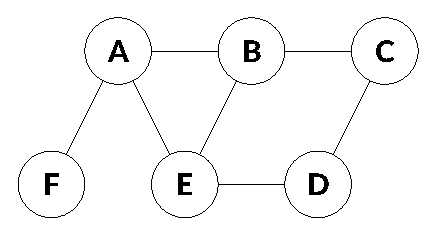
\includegraphics[width=0.98\linewidth]{figures/quickfire_north_audition_validbfs.eps}
}

\begin{multicols}{5}
    \begin{enumerate}[label={$\Circle$}]
        \item \verb|ABCDEF|
        \item \verb|EABDFC|
        \item \verb|BEADCF|
        \item \verb|EABDCF|
        \item \verb|FAEDBC|
    \end{enumerate}
\end{multicols}

\question{}

จงศึกษาตัวอย่างโจทย์ดังต่อไปนี้ แล้วจึงแก้โจทย์ในช่วงท้ายของคำถาม

\smallskip\noindent
\textbf{\uline{ตัวอย่าง}}\; จากนิพจน์ (expression) ทางคณิตศาสตร์ต่อไปนี้
\[
    \mathrm{5 - 2 + 8 - 4 - 3}
\]

หากเราเติมวงเล็บในนิพจน์ข้างต้นกี่คู่ก็ได้เพื่อ\uline{เปลี่ยนกลุ่มการบวกหรือการลบ}เท่านั้น\hrsp%
\sidenote{%
    \textbf{ยกตัวอย่าง} เช่น
    \begin{itemize}
    \item $\mathrm{5 - (2 + 8) - 4 - 3 = -12}$
    \item $\mathrm{5 - (2 + 8 - 4 - 3) = 2}$
    \item $\mathrm{5 - (2 + 8 - (4 - 3)) = -4}$
    \end{itemize}
    \textbf{หมายเหตุ}\; แต่\uline{ไม่อนุญาต}ให้มีการคูณเกิดขึ้นจากการเติมวงเล็บในนิพจน์ที่กำหนดให้ เช่น
    \begin{itemize}
    \item $\mathrm{5 - 2 + 8 (-4)(-3) = 99}$
    \end{itemize}
}
จะทำให้ผลลัพธ์สุดท้ายที่ได้ต่างออกไป\;
แต่วิธีการเติมวงเล็บที่ทำให้ผลลัพธ์สุดท้ายที่ค่า\uline{มาก} \uline{ที่สุด}คือ
\[
    \mathrm{5 - 2 + 8 - (4 - 3) = 10}
\]

\noindent
\textbf{\uline{โจทย์}}\; จงพิจารณานิพจน์ที่เป็นโจทย์ดังต่อไปนี้แล้วตอบว่า 
จะเติมวงเล็บลงในนิพจน์นี้เพื่อเปลี่ยนกลุ่มการลบ 
และให้ผลลัพธ์สุดท้ายมีค่ามากที่สุด จะได้ค่าเท่าใด?
\[
    \mathrm{0 - 1 - 2 - 3 - 4 - 5 - 6 - 7 - 8 - 9 - 10}
\]

\question{}

จงพิจารณานิพจน์ที่เป็นโจทย์ดังต่อไปนี้แล้วตอบว่า จะเติมวงเล็บลงในนิพจน์นี้เพื่อ\uline{เปลี่ยนกลุ่มการบวกหรือการลบ}
และให้ผลลัพธ์สุดท้ายมีค่ามากที่สุด จะได้ค่าเท่าใด?
\[
    \mathrm{10 - 9 - 8 - 7 - 6 + 5 - 4 - 3 - 2 - 1} 
\]


\newpage
\question{\label{q:quickfire_south_regional_reverseshuffle}}

จงพิจารณาโปรแกรมดังต่อไปนี้
\begin{lstlisting}
function mystery_<%\ref*{q:quickfire_south_regional_reverseshuffle}%>(A[0...n-1])
    # A <%\codecmt คือ%> 0-indexed array  
    n := A.length()
    for i := 0 to n-1
        for j := n downto i + 1
            swap values between A[i] and A[j]
        end
    end
    return A
end
\end{lstlisting}

จงหา array \lstinline{A} ที่เมื่อป้อนเป็น input ให้แก่โปรแกรมข้างต้นแล้ว
จะได้ output ออกมาเป็น array ที่มีค่า \lstinline{[1, 2, 3, 4]}

\question{}

มีกล่องอยู่ 75 ใบ
\begin{itemize}
\item กล่องแต่ละใบถูกล็อกไว้ด้วยแม่กุญแจที่แตกต่างกันทั้งหมด
\item กุญแจสำหรับแม่กุญแจแต่ละอัน ถูกบรรจุซ่อนอยู่ในกล่องใบอื่น ๆ (แปลว่ากุญแจที่จะเปิดกล่อง X จะอยู่ในกล่องอื่นซึ่งไม่ใช่ X)
\item นอกจากนั้น แต่ละกล่องมีกุญแจอยู่ข้างในเพียงดอกเดียว
\item การเปิดกล่องหนึ่งกล่องมีได้สองวิธีคือ 1.~ทำลายแม่กุญแจ หรือ 2.~ใช้กุญแจไข
\end{itemize}

หากเราต้องการเปิดกล่องทุกใบออกทั้งหมด โดยที่ทำลายแม่กุญแจให้น้อยที่สุด\;
ในกรณีที่เลวร้ายที่สุดจะต้องทำลายแม่กุญแจอย่างน้อยกี่กล่องจึงจะเปิดกล่องได้ครบ 75 ใบ?

\question{}

เรานิยาม \textbf{Proper binary tree} คือต้นไม้ทวิภาคที่ทุกโหนดมีโหนดลูกเป็นจำนวน 0 หรือ 2 โหนดพอดีเท่านั้น\;
(กล่าวคือทุกโหนดที่เป็น Internal/Non-leaf Node จะต้องมีโหนดลูก 2 โหนดพอดี)

สมมติว่าเรามี Programming Library ตัวหนึ่งที่สามารถจัดการข้อมูลที่มีโครงสร้างเป็น Proper binary tree 
ซึ่งมีรายละเอียดดังต่อไปนี้

\begin{description}
    \item[Data type.] โหนดแต่ละโหนดของ Proper binary tree จะมี data type ที่มีชื่อว่า 
        \lstinline{Node} ซึ่งแบ่ง subtype ได้ 2 แบบย่อย ดังนี้
        \begin{itemize}
            \item \lstinline|Leaf{value: Integer}| \\
                เป็น Leaf node ซึ่งประกอบด้วยข้อมูล 1 อย่าง ซึ่งก็คือจำนวนเต็มภายในโหนด
            \item \lstinline|Internal{left: Node, right: Node, value: Integer}| \\
                เป็น Non-leaf node ซึ่งประกอบด้วยข้อมูลทั้งสิ้น 3 อย่าง ได้แก่
                1.~Subtree ทางซ้าย 2.~Subtree ทางขวา 
                และ 3.~ข้อมูลจำนวนเต็มภายในโหนด ตามลำดับ
        \end{itemize}
    \item[Library function.] กำหนดให้ฟังก์ชัน \lstinline{compute} 
        รับข้อมูลต้นไม้ประเภท \lstinline{Node} และฟังก์ชันอื่น ๆ อีก 2 ฟังก์ชัน (ดูโค้ดด้านล่างประกอบ) 
        เพื่อประมวลผลข้อมูลต้นไม้ดังกล่าว ซึ่งสามารถเขียนเป็น pseudocode ได้ดังต่อไปนี้
\end{description}

\newpage
\vspace*{-2\baselineskip}
\begin{fullwidth}%
\begin{lstlisting}[language=pseudocode]
function compute(tree: Node,
                 leaf_transformer: function,        # signature: Integer -> T
                 internal_transformer: function):   # signature: T, T, Integer -> T
    if tree matches Leaf{value} then:
        return leaf_transformer(value)
    else if tree matches Internal{left, right, value} then:
        return internal_transformer(
            compute(left, leaf_transformer, internal_transformer), 
            compute(right, leaf_transformer, internal_transformer), 
            value
        )
    end
end
\end{lstlisting}
\end{fullwidth}

\noindent%
\textbf{\uline{โจทย์}}\; สมมติว่าเรามีข้อมูล Proper binary tree ที่เก็บอยู่ในตัวแปรชื่อ \lstinline{data}
แล้วโปรแกรมในข้อใดต่อไปนี้จะนับจำนวนโหนดทั้งหมดภายในต้นไม้ (ทั้ง Leaf และ Non-leaf) 
ภายในตัวแปร \lstinline{data} ดังกล่าวได้ถูกต้อง?\hrsp%
\sidenote[][-2\baselineskip]{%
    \textbf{หมายเหตุ}\; ยกตัวอย่าง syntax ของฟังก์ชันนิรนาม เช่น \lstinline{lambda(x, y) -> (x + y)/2} 
    คือฟังก์ชันที่หาค่าเฉลี่ยของตัวเลข input argument สองตัว
}

\begin{fullwidth}
\bigskip
\begin{enumerate}[label={$\Circle$}]
    \item \lstinline{compute(data, lambda(v) → v, lambda(l, r, v) → l + r)}
    \item \lstinline{compute(data, lambda(v) → v, lambda(l, r, v) → l + r) * 2}
    \item \lstinline{compute(data, lambda(v) → v, lambda(l, r, v) → l + r) * 2 + 1}
    \item \lstinline{compute(data, lambda(v) → v, lambda(l, r, v) → l + r) * 2 - 1}
    \item \lstinline{compute(data, lambda(v) → v, lambda(l, r, v) → l + r + v)}
    \item \lstinline{compute(data, lambda(v) → v, lambda(l, r, v) → l + r + v) * 2}
    \item \lstinline{compute(data, lambda(v) → v, lambda(l, r, v) → l + r + v) * 2 + 1}
    \item \lstinline{compute(data, lambda(v) → v, lambda(l, r, v) → l + r + v) * 2 - 1}
    \item \lstinline{compute(data, lambda(v) → 1, lambda(l, r, v) → l + r) * 2}
    \item \lstinline{compute(data, lambda(v) → 1, lambda(l, r, v) → l + r) * 2 + 1}
    \item \lstinline{compute(data, lambda(v) → 1, lambda(l, r, v) → l + r) * 2 - 1}
    \item \lstinline{compute(data, lambda(v) → 1, lambda(l, r, v) → l + r + 1) * 2}
    \item \lstinline{compute(data, lambda(v) → 1, lambda(l, r, v) → l + r - 1) * 2}
    \item \lstinline{compute(data, lambda(v) → 0, lambda(l, r, v) → l + r) * 2}
    \item \lstinline{compute(data, lambda(v) → 0, lambda(l, r, v) → l + r) * 2 + 1}
    \item \lstinline{compute(data, lambda(v) → 0, lambda(l, r, v) → l + r) * 2 - 1}
    \item \lstinline{compute(data, lambda(v) → 0, lambda(l, r, v) → l + r + 1) * 2}
    \item \lstinline{compute(data, lambda(v) → 0, lambda(l, r, v) → l + r - 1) * 2}
\end{enumerate}
\end{fullwidth}


\newpage
\question{}

สมมติว่าเราต้องการสร้างรูปเรขาคณิตใหม่ โดยนำชิ้นส่วนจัตุรัสขนาด 1 ตารางหน่วยอย่างน้อย 1 ชิ้นมาประกอบกัน โดยมีเงื่อนไขดังต่อไปนี้
\begin{itemize}
    \item รูปเรขาคณิตใหม่จะต้องไม่มีชิ้นส่วนที่แยกจากกัน
        (ยกตัวอย่างเช่นรูป \textbf{(c)} \uline{ใช้ไม่ได้})
    \item ชิ้นส่วนจัตุรัสสองชิ้นที่แตะกันเฉพาะตำแหน่งมุม ถือว่าเป็นชิ้นส่วนที่แยกจากกัน
        (รูปตัวอย่าง \textbf{(d)} \uline{ใช้ไม่ได้})
    \item รูปเรขาคณิตใหม่จะต้องไม่มีรูหรือช่องว่างภายในรูปปิด 
        (ตัวอย่างเช่นรูป \textbf{(e)} \uline{ใช้ไม่ได้})
    \item รูปเรขาคณิตใหม่จะต้องมีทุกด้านยาว 1 หน่วยเท่านั้น 
        (เช่นรูป \textbf{(f)} หรือ \textbf{(g)} \uline{ใช้ไม่ได้} 
        เพราะมีบางด้านยาว 0.5 หน่วย หรือ 2 หน่วย)
\end{itemize}
\marginnote[-8\baselineskip]{%
    \centering
    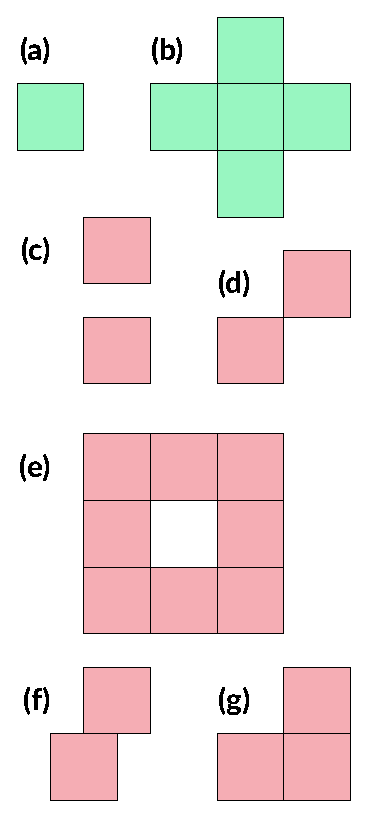
\includegraphics[width=0.70\linewidth]{figures/quickfire_central_audition_squaretiling.eps}
}

สังเกตว่า หากเรามีชิ้นส่วนจัตุรัส 1 ชิ้นพอดี หรือ 5 ชิ้นพอดี
(จากรูปตัวอย่าง \textbf{(a)} และ \textbf{(b)} ตามลำดับ) 
เราสามารถสร้างรูปเรขาคณิตที่สอดคล้องกับเงื่อนไขข้างต้นได้\;
อย่างไรก็ดี เรา\uline{ไม่สามารถ}สร้างรูปเรขาคณิตตามเงื่อนไขดังกล่าวได้เลย 
หากเรามีชิ้นส่วนจัตุรัสเพียง 2 หรือ 3 หรือ 4 ชิ้นเท่านั้น

จงหาจำนวนชิ้นส่วนจัตุรัสที่\hrsp\uline{มากที่สุด}{\hrsp}ที่\hrsp\uline{ไม่สามารถ}{\hrsp}นำมาประกอบเป็นรูปเรขาคณิตตามเงื่อนไขข้างต้นได้

\question{}

สมมติว่ามีไพ่สำรับมาตรฐาน \uline{2 สำรับ} สำรับละ 52 ใบ รวมทั้งสิ้น 104 ใบ วางกองไว้รวมกันโดยไม่เรียงลำดับ

\begin{itemize}
    \item \uline{ไพ่ 1 สำรับ} มีชุดตัวเลขทั้งสิ้น 13 ชุด (2, 3, 4, \ldots, 10, J, Q, K, A) ชุดละ 4 ใบ
    \item \uline{ไพ่ตอง} คือ ไพ่สามใบที่ชุดตัวเลขเหมือนกันเช่น 2, 2, 2 หรือ K, K, K
\end{itemize}

เราจะต้องหยิบไพ่ในกองดังกล่าวอย่างสุ่ม\uline{อย่างน้อยกี่ใบ} จึงจะรับประกันว่าในบรรดาไพ่ที่เราหยิบมาจะ\uline{มีไพ่ตองอย่างน้อย 1 ชุด}?
\question{\label{q:quickfire-northeast-regional-whatm}}

จงพิจารณาโปรแกรมดังต่อไปนี้
\begin{lstlisting}
function mystery_<%\ref*{q:quickfire-northeast-regional-whatm}%>(A[0...n-1]):
    # A <%\codecmt คือ%> 0-indexed array <%\codecmt ของจำนวนเต็ม%>
    n = A.length()
    result = 0
    for i := 0 to n-1 do:
        if A[i] < result then:
            result := A[i]
        end
    return result
end
\end{lstlisting}

จงหาผลลัพธ์ของการรันโปรแกรม \lstinline{mystery_}%
\texttt{\small\ref*{q:quickfire-northeast-regional-whatm}}%
\lstinline{([9, 43, 214, 1, 5])}


\newpage
\question{}

คำถามเกี่ยวกับอัลกอริทึม Depth-first search (DFS)

\smallskip\noindent
\textbf{\uline{ตัวอย่าง}}\; พิจารณากราฟที่มีลักษณะเป็น grid ขนาด $\mathrm{3} \times \mathrm{3}$ 
ดังที่แสดงทางด้าน%
{\ifodd\thepage{ขวา}\else{ซ้าย}\fi} 
หากเราใช้อัลกอริทึม Depth-first search (DFS) กับกราฟนี้โดยเริ่มต้นจากโหนดใดก็ได้ 
เราจะได้ Maximum recursion depth เท่ากับ 9 ดังที่แสดงด้วยเส้นสีฟ้า

\begin{center}
    \bigskip
    \includegraphics[scale=0.6]{figures/quickfire_north_regional_recursiondepth_01.eps}
\end{center}
% \marginnote[-2\baselineskip]{%
%     \centering
%     \includegraphics[scale=0.6]{figures/quickfire_north_regional_recursiondepth_01.eps}\\
%     รูปประกอบกรณี\uline{ตัวอย่าง}
% }

\noindent
\textbf{\uline{โจทย์}}\; จงหา Maximum recursion depth ที่เป็นไปได้ 
หากเราสามารถใช้อัลกอริทึม Depth-first search จากโหนดใดก็ได้ในกราฟต่อไปนี้
\begin{center}
    \bigskip
    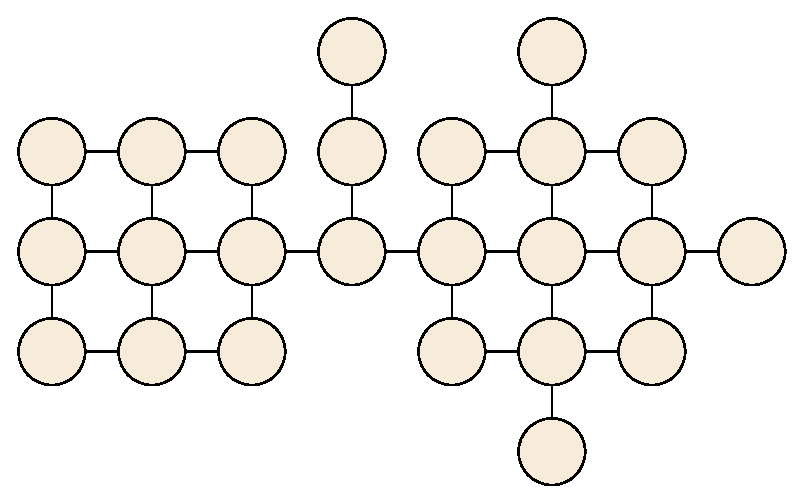
\includegraphics[scale=0.6]{figures/quickfire_north_regional_recursiondepth_02.eps}
\end{center}

\question{} 

เรากำหนดให้มีกล่องจำนวนหนึ่งวางอยู่บนโต๊ะ ซึ่งกล่องบางใบอาจจะถูกซ้อนอยู่ภายในกล่องใบอื่นก็ได้ และมีเงื่อนไขเพื่อความชัดเจนว่า
\begin{itemize}
    \item \uline{ถ้า}กล่อง X ถูกซ้อนในกล่อง Y \uline{และ}กล่อง Y ถูกซ้อนในกล่อง Z 
        \uline{แล้ว}กล่อง X จะถือว่าถูกซ้อนในกล่อง Z ด้วย
    \item \uline{ถ้า}กล่อง X ถูกซ้อนในกล่อง Y \uline{แล้ว}กล่อง Y จะไม่ถูกซ้อนในกล่อง X
\end{itemize}
นอกจากเงื่อนไขข้างต้นนี้ เรากำหนดนิยามเพิ่มเติมดังต่อไปนี้
\begin{quote}
    \textbf{\uline{นิยาม}}\; หากกำหนดให้ $B$ เป็นสัญลักษณ์ที่สื่อถึงรูปแบบของการจัดวางกล่องบนโต๊ะตามเงื่อนไขที่กำหนดให้ 
    แล้วสัญลักษณ์ $B[n]$ จะหมายถึง ``จำนวนของกล่องทั้งหมดบนโต๊ะที่มีกล่องอื่น ๆ จำนวน $n$ ใบซ้อนอยู่ภายใน''

    \marginnote{%
        \centering
        
\includegraphics[width=0.98\linewidth]{figures/quickfire_central_regional_nestbox.eps}\\
        รูปตัวอย่างการจัดวางกล่อง $B_0$
    }

    ยกตัวอย่างเช่น สมมติว่า $B_0$ คือการจัดวางกล่อง 5 ใบบนโต๊ะรูปแบบหนึ่ง ดังที่แสดงทางด้าน\ifpageodd{ขวา}{ซ้าย}มือนี้
    เราสามารถบอกได้ว่า $B_0[1] = \mathrm{2}$ (กล่องสีฟ้า), $B_0[2] = \mathrm{0}$, 
    $B_0[3] = \mathrm{0}$ และ $B_0[4] = \mathrm{1}$ (กล่องสีแดง) ฯลฯ
\end{quote}

\noindent
\textbf{\uline{โจทย์}}\; จงคำนวณว่าสำหรับการจัดวางกล่อง $B_1$ \uline{ในรูปแบบใด\,ๆ} 
ที่สอดคล้องกับเงื่อนไขว่า $B_1[1] = \mathrm{5}$,\, $B_1[2] = \mathrm{4}$,\, $B_1[3] = \mathrm{3}$,\, 
$B_1[4] = \mathrm{2}$ และ $B_1[5] = \mathrm{1}$ จะต้อง\uline{มีจำนวนกล่องรวม}ทั้งหมดอย่างน้อยกี่ใบ?


\newpage
\question{\label{q:quickfire_central_audition_sortbetweenintro}}

กำหนดให้มีฟังก์ชันหนึ่ง \lstinline{sort_between(L, p, q)}    ซึ่งมีสเปกดังนี้ 
\begin{itemize}
    \item ข้อมูล input \lstinline{L} เป็น 0-indexed array ของจำนวนชุดหนึ่ง
    \item ข้อมูล input \lstinline{p} และ \lstinline{q} เป็น index 
        ภายใน array \lstinline{L} โดยที่มีเงื่อนไขว่า \\
        \lstinline{0 <= p <= q < L.length()}
    \item ข้อมูล output ของ \lstinline{sort_between(L, p, q)} 
        จะเป็น array ใหม่ ซึ่งเกิดจากการจัดเรียงจำนวนบางจำนวนใน array \lstinline{L} เดิม 
        ตั้งแต่ตำแหน่ง \lstinline{p} ถึงตำแหน่ง \lstinline{q} จากน้อยไปมาก
        และจำนวนในตำแหน่งอื่น ๆ นอกเหนือจากนี้ยังคงเดิม
\end{itemize}

\noindent
\textbf{\uline{ยกตัวอย่าง}}\; ถ้ากำหนดให้ \lstinline{L_0 = [4, 2, 7, 3, 8, 1, 5]}
แล้วเมื่อเรียกฟังก์ชัน \lstinline{sort_between(L_0, 2, 4)}  
จะได้ output เป็น \lstinline{[4, 2, 1, 3, 7, 8, 5]}

\medskip\noindent
\textbf{\uline{โจทย์}}\; สมมติว่าเรามี array \lstinline{L_1} 
ซึ่งประกอบไปด้วยจำนวนทั้งสิ้น 250 จำนวน โปรแกรมในข้อใดต่อไปนี้\hrsp\uline{ไม่รับประกัน}\hrsp%
ว่าสามารถเรียงลำดับจำนวนทุกจำนวนภายใน array ได้ทั้งหมด?
\begin{enumerate}[label={$\Circle$}]
\item \lstinline{sort_between(L_1, 0, 249)}
\item
    \lstinline{sort_between(L_1, 0, 199)} \\
    \lstinline{sort_between(L_1, 150, 249)} \\
    \lstinline{sort_between(L_1, 0, 199)}
\item 
    \lstinline{sort_between(L_1, 0, 199)} \\
    \lstinline{sort_between(L_1, 50, 249)} \\
    \lstinline{sort_between(L_1, 0, 149)}
\item 
    \lstinline{sort_between(L_1, 100, 249)} \\
    \lstinline{sort_between(L_1, 0, 149)} \\
    \lstinline{sort_between(L_1, 50, 249)}
\item 
    \lstinline{sort_between(L_1, 150, 249)} \\
    \lstinline{sort_between(L_1, 0, 199)} \\
    \lstinline{sort_between(L_1, 150, 249)}
\end{enumerate}

\question{}

กำหนดให้มีฟังก์ชันหนึ่ง \lstinline{sort_between(L, p, q)} 
ซึ่งมีสเปกเหมือนกับคำถามที่แล้ว (ดู\autoref{q:quickfire_central_audition_sortbetweenintro})

เราจะนำฟังก์ชัน \lstinline{sort_between} ดังกล่าวนี้มาใช้งานเพื่อเขียนฟังก์ชันใหม่ที่มีชื่อว่า
\lstinline{slider_sort_between} ซึ่งมีกระบวนการทำงานดังต่อไปนี้
\begin{lstlisting}
function slider_sort_between(L, k):
    n := L.length()
    for i := 0 to n-k do:
        # <%\codecmt เรียงลำดับจำนวนที่ติดกัน%> k <%\codecmt จำนวนใน%> array L
        # <%\codecmt ตั้งแต่ตำแหน่งที่%> i <%\codecmt จนถึงตำแหน่งที่%> i-k+1
        sort_inplace(L, i, i+k-1)
    end
end
\end{lstlisting}

สมมติว่าเรามี array \lstinline{L_1} ซึ่งประกอบไปด้วยจำนวนทั้งสิ้น 250 จำนวน\;
เป้าหมายคือเราต้องการเรียงลำดับจำนวนทุกจำนวนภายใน array นี้ด้วยการเรียกใช้งานคำสั่ง
\begin{center}
    \lstinline{L_1 := slider_sort_between(L_1, k=25)}
\end{center}
นี้\uline{ซ้ำ\;ๆ\;กัน}อย่างต่อเนื่อง จนกว่าจำนวนใน array \lstinline{L_1} จะเรียงลำดับทั้งหมด\;
อยากทราบว่าเราจะต้องรันคำสั่งข้างต้นนี้\uline{อย่างน้อย}กี่รอบ
จึงเพียงพอที่จะรับประกันว่าค่าทั้งหมดของ array \lstinline{L_1} เรียงลำดับจากน้อยไปมาก?

\question{}

คำถามเกี่ยวกับการลากเส้นรูปปิดตามโครงสร้างที่กำหนดให้

\smallskip\noindent
\textbf{\uline{ตัวอย่าง}}\; จากรูปที่แสดงทาง\ifpageodd{ขวา}{ซ้าย}มือนี้
\marginnote{%
    \centering
    
\includegraphics{figures/quickfire_central_regional_closedshapearea_01.eps}
}
มีโครงสร้างเรขาคณิตที่เรียงตัวเป็นสามเหลี่ยมด้านเท่าย่อย ๆ หลายรูปประกอบกัน
โดยที่สามเหลี่ยมย่อยแต่ละรูปมีพื้นที่รูปละ 1 ตารางหน่วย

จากโครงสร้างเรขาคณิตรูปนี้ เราจะพยายามลากเส้นภายในโครงสร้างที่กำหนดให้ข้างต้น โดยมีเงื่อนไขว่า
\begin{itemize}
\item เราจะต้องลากเส้นเพียงเส้นเดียว ผ่านจุดยอดให้ครบทุกจุด แล้วกลับมายังจุดเริ่มต้น กลายเป็นรูปปิด
\item จุดยอดแต่ละจุดจะต้องถูกเยือน 1 ครั้งพอดี ไม่ขาดและไม่เกิน
\item เส้นทุกเส้นที่ลากผ่านจะต้องมีเค้าโครงเดิมจากเส้นสีเทาที่กำหนดให้จากรูปดั้งเดิม
\item รูปปิดที่เกิดขึ้นจะต้องมี\uline{พื้นที่ภายในมากที่สุด}เท่าที่เป็นไปได้
\end{itemize}

\marginnote{%
    \centering
    
\includegraphics{figures/quickfire_central_regional_closedshapearea_02.eps}
}

รูปที่สองที่ปรากฏทางด้าน\ifpageodd{ขวา}{ซ้าย}มือนี้
แสดงหนึ่งในวิธีที่เราสามารถลากเส้นรูปปิดภายในโครงสร้างเรขาคณิต (ดังที่แสดงในรูปแรก)
ที่สอดคล้องกับเงื่อนไขที่กล่าวมาข้างต้นได้ทั้งหมด ซึ่งรูปปิดดังกล่าวจะได้พื้นที่ภายในรวม 8 ตารางหน่วย\;
(\textbf{หมายเหตุ:} อาจมีวิธีลากเส้นวิธีอื่น~ๆ ที่ทำให้ได้พื้นที่ขนาดเท่ากัน)

\medskip\noindent
\textbf{\uline{โจทย์}}\; 
จงหาว่าในรูปต่อไปนี้ เราจะลากเส้นสร้างรูปปิดตามเงื่อนไขเดียวกันให้ได้พื้นที่ภายในมากที่สุด จะได้พื้นที่เท่าใด?
\begin{center}
    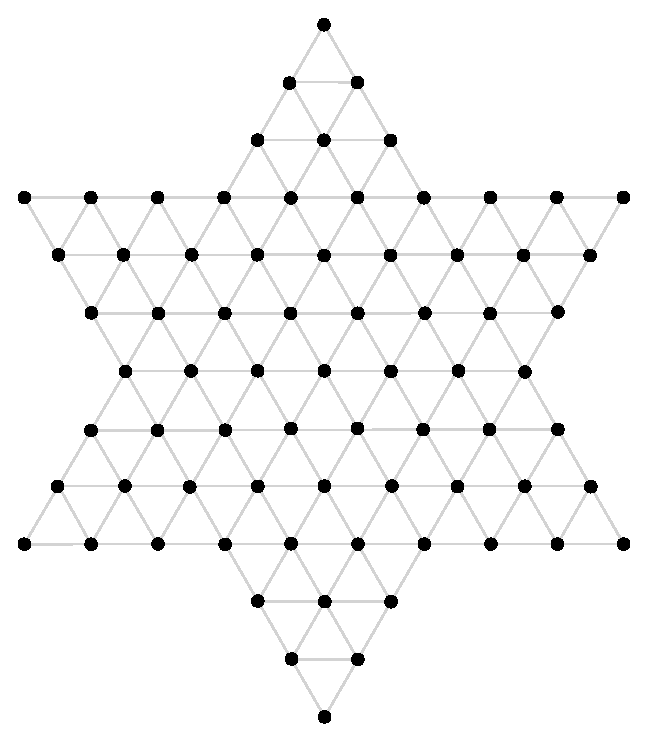
\includegraphics[width=0.7\linewidth]{figures/quickfire_central_regional_closedshapearea_03.eps}
\end{center}

\newpage
\question{}

จงพิจารณานิยามของลำดับ (ordering) ในการท่องต้นไม้ค้นหาแบบทวิภาค (Binary search tree) 
ที่แตกต่างกันดังต่อไปนี้

\marginnote{%
    \textbf{ตัวอย่าง} เช่นจากรูปต้นไม้ตัวอย่างนี้

    \begin{center}
        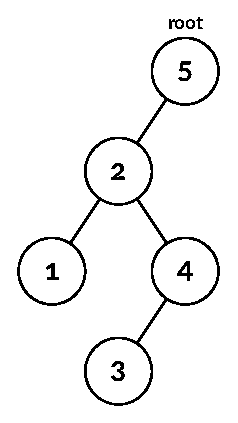
\includegraphics[width=0.6667\linewidth]{figures/quickfire_central_regional_bfsdfs.eps}
    \end{center}

    \begin{itemize}
        \item จะมี Pre-order traversal ordering เป็น $[\mathrm{5, 2, 1, 4, 3}]$
        \item และจะมี Breadth-first search ordering ได้สองรูปแบบ 
            ได้แก่ $[\mathrm{5, 2, 1, 4, 3}]$ และ $[\mathrm{5, 2, 4, 1, 3}]$
    \end{itemize}
}

\begin{itemize}
    \item \textbf{Pre-order traversal}
    ของโครงสร้างข้อมูลต้นไม้ค้นหาทวิภาค (Binary search tree) คือการใช้อัลกอริทึม 
    Depth-first search (DFS) เพื่อประมวลผลโหนดแต่ละโหนดของต้นไม้หนึ่งตามลำดับดังต่อไปนี้ 
    (โดยนับเริ่มต้นจากราก (root) ของต้นไม้)

    \begin{enumerate}
    \item compute โหนดตัวเอง
    \item recursively compute โหนดในกลุ่ม Subtree ทางซ้ายของโหนดตัวเอง
    \item recursively compute โหนดในกลุ่ม Subtree ทางขวาของโหนดตัวเอง
    \end{enumerate}

    \item \textbf{Breadth-first search ordering} 
    ของโครงสร้างข้อมูลต้นไม้ทวิภาค (Binary tree) คือลำดับการท่องต้นไม้ตามอัลกอริทึม 
    Breadth-first search (BFS) (\textbf{หมายเหตุ:} โดยมีเงื่อนไขกำหนดให้เริ่มต้นจากรากของต้นไม้) 
\end{itemize}

\noindent
\textbf{\uline{โจทย์}} สมมติว่ามีต้นไม้ค้นหาแบบทวิภาค (Binary search tree) $T$ อยู่ต้นหนึ่ง
ซึ่งพบว่ามีลำดับ Pre-order traversal เป็น $[\mathrm{7, 2, 1, 4, 3, 6, 5, 9, 8, 10, 11}]$\;
อยากทราบว่าต้นไม้ $T$ นี้จะมี Breadth-first search (BFS) ordering 
ที่เริ่มต้นจากรากได้ต่างกันทั้งหมด\uline{กี่รูปแบบ}?

\question{}

สมมติว่าครอบครัวหนึ่ง มีลูกทั้งสิ้น 5 คน ได้แก่ 
Dijkstra (D), Hopper (H), Lovelace (L), Neumann (N) และ Shannon (S) 
ซึ่งไม่เรียงลำดับใด ๆ ทั้งสิ้น

ต่อไปนี้จะเป็นคำบอกเล่าของแม่ 7 ประโยค ซึ่งมี \uline{1 ประโยคเท่านั้นที่เป็นเท็จ}

\begin{enumerate}
\item Hopper มีอายุน้อยกว่า Shannon
\item Dijkstra มีอายุน้อยกว่า Lovelace
\item Shannon มีอายุน้อยกว่า Neumann
\item Hopper มีอายุน้อยกว่า Dijkstra
\item Lovelace มีอายุน้อยกว่า Shannon
\item Shannon มีอายุน้อยกว่า Dijkstra
\item Neumann มีอายุน้อยกว่า Lovelace
\end{enumerate}

\noindent
จงตอบคำถามว่า 1. ประโยคข้างต้นใดเป็นเท็จ และ 2. ใครเป็นพี่คนโต


